\documentclass{article}
\usepackage[utf8]{inputenc}
\usepackage[spanish]{babel}
\usepackage{graphicx}
\usepackage{geometry}
\usepackage{multicol}
\usepackage{amsmath}
\usepackage{amsthm,amsfonts,amssymb}%paquetes AMS
\usepackage{hyperref}

\begin{document}

\pagestyle{empty}
%\afterpage{\blankpage}
\begin{center}
\begin{figure}[h]
\centering


\end{figure}
\Large
\hrule
\vspace{4mm}
\textbf{Notas del Curso de Creatividad Financiera}\\

\vspace{4mm}
\hrule
\large
\vfill
Autor\\

Wilson Eduardo Jerez Hernández \\
\vfill
Profesora\\

Liliana Zamacona
\vfill
Platzi\\
Escuela de Finanzas e Inversiones\\
Curso de Creatividad Financiera\\
\end{center}
\newpage
\newpage
\addtocontents{toc}{\hfill \textbf{Página} \par}
\tableofcontents
\newpage

\section{Lo que aprenderás para tener creatividad financiera}
este curso es un montón de historias, este curso no es una formula magiga.
tener un \textbf{Diario de innovación, aprendizaje y creatividad}
\textbf{Ordena la información}
\begin{enumerate}
    \item Utilizar de manera constante y
    habitual un diario donde se escriban
    todas las ideas de negocio
    \item Tratar de desarrollar lo más posible
    cada idea.
    \item Medir, evaluar y asimilar este
    aprendizaje para aplicarlo en futuros
    desarrollos.
\end{enumerate}


\section{Historias que inspiran}
la resilencia es lo que nos saca adelante.
para poder pararte rapidamente.
por ejemplo \textbf{rosario marín} tambien \textbf{Shaquem Griffin}
\begin{enumerate}
    \item gente que nuca paraa de aprenderno importa la edad ni las condiciones
\end{enumerate}

\section{La importancia de la creatividad y resilencia financiera}
\text{Resiliencia Financiera}
\begin{enumerate}
    \item Reinventa tus ingresos
    una y otra vez.
    \item  A veces estamos arriba,
    a veces estamos abajo.
    \item  Comprende los entornos
    económicos.
\end{enumerate}
la vida es un ciclo krnal 

\section{Florecer en la crisis}
Unos lloran, otros venden pañuelos.
por ejemplo con la crisis de covid muchos aprovecharon la mueva realidad.

\section{Detén el pánico financiero que existe en tu mente}
una mente cansada no es una mente creativa.
La mente es caótica, busacará los peores escenarios.
tendemos a exagerar.
la mente no tiene sistema de depuración.
"Una persona puede
mantener un
pensamiento que le
lastima durante toda
su vida y dejarlo ahí
sin hacer nada por ello."
por tanto te corresponde a ti limpiarte. \textbf{Entrena tu mente}
como tomar el cursos de inteligencia emocional.

\section{Trampas que nos detienen en nuestro crecimiento financiero}

\textbf{pensamiento critico}
El pensamiento crítico es la capacidad
manifestada por el ser humano para
analizar y evaluar la información existente
respecto a un tema determinado.
"las pérdidad nos hacen estar mentalmente derrotados y si no tenemos un pensamiento crítico,
pueden volverse una carga tan pesada que vamos a permitir que nos definan." - john C Maxwell
\textbf{los errores no te definen}.
11 trampas \begin{enumerate}
    \item Error.tengo miedo a equivocarme.
    \item comparación. alguien puede hacerlo mejor que yo.
    \item fatiga. que pereza we xd 
    \item momento oportuno. este no es un buen momento.
    \item inspiración. no me siento con ganas.
    \item perfección. hay una mejor forma de hacerlo.
    \item racionalización. talvez este negocio no es importante, a nadie le va a importar, aveces tanto pensar nos aleja de nuestros sueños.
    \item expectativa. Quisiera que esto fuera mas grande, ser el mejor, tantas conversaciones con nosotros mismos.
    \item Juscia. esto no me corresponde, pensamos que la vida es injusta.
    \item vergüenza. si fallo que van a pensar de mi. 
    \item Autoimagen. que van a pensar de mi. esta es una de las trampas que mas nos duele.
\end{enumerate}
\section{Reconocer patrones de conducta financieros}
hay ciertos pratones de conducta que es probable que heredemos.
preguntale a tus antepasados xd.
\textbf{Reflexiona}
\begin{enumerate}
    \item ¿como reaccionaron?
    \item ¿Qué fue lo que aprendieron?
    \item ¿Los volvieron a repeir?
    \item ¿Qué patrones de conductas se repiten continuamente?
\end{enumerate}
\textbf{importante no juzgues}.
No le des poder a tu entorno social.
\begin{enumerate}
    \item ¿tu entorno afecta o aumenta tu estrés financiero?
    \item ¿sientes culpa por pensar diferente que el resto de las perosanas que amas?
    \item ¿Estás rodeado de múltiples facores y detonantes que estimulan el pensamiento de que etsamos en crisis?
\end{enumerate}
por que nosotros vamos a querer pentenecer a nuestra tribu.
es una trampa pero inconcientes.
\textbf{checklist para una mente blindada.} 
\begin{enumerate}
    \item establece límites.
    \item sé altamente productivo.
    \item practica la atención enfocada al menos 1 vez al día. 
    \item cuestiónate al final de cada día.
    \item consume información poderosa para tu desarrollo.
\end{enumerate}
\section{El túnel de la escasez}
haz sentido que estas atrapado en un lugar y no puedes salir.
\textbf{Mentalidad de escasez}
¿como nos afecta en la toma de decisiones, ejecucuión innovación y creatividad?
la creatividad radica en tu mente.
\begin{center}
    "si no se controla, la escasez puede tner efectetos nocivos en el performance de las perosanas.
    La buena noticia es que los líderes tienen la opurtiunidad de ayudar a prevenir la "mentalidad de escasez"
    antes de que ocurra"
\end{center}
\textbf{El túnel}
La escasez o carencia de un determinado recurso reduce nuestra capacidad cognitiva.
El cerebro se obsesiona. \textbf{ESTAS ENTRANDO EN UN TÚNEL}
\begin{center}
    \textbf{LA TRAMPA DE LA ESCASEZ}\\
        La escasez de la sensación de tner más necesidades que recursos.
        Nos lleva a tener visión de túnel, lo que nos hace enfocarnos en algo, excluyendo y negando
        otros cosas importantes.\\
\end{center}
\newpage
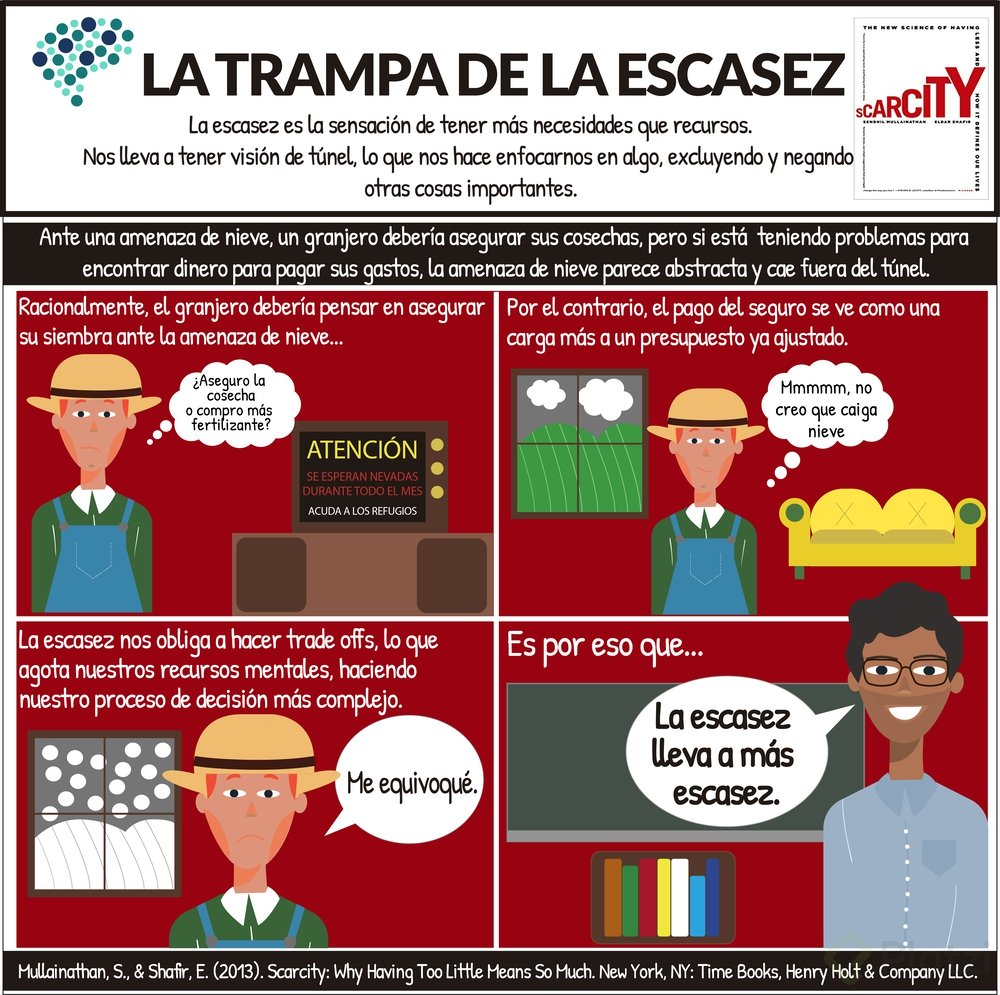
\includegraphics[scale=0.5]{imagenes/infografia-sobre-la-trampa-de-la-escasez.png}


\end{document}